\documentclass[12pt]{ctexart} % 使用 ctexart 文档类支持中文

\usepackage{fancyhdr} % 奇特的 header
\usepackage{xcolor} % 更多颜色

\usepackage[utf8]{inputenc} % 支持 UTF8 字符
\usepackage{xeCJK} % 支持中文排版,已经包含在 ctexart 中
\usepackage{fontspec} % 字体设置
\usepackage{geometry} % 页面布局
\usepackage{titlesec} % 自定义标题样式
\usepackage{setspace} % 设置行距

\usepackage[colorlinks,linkcolor=black,urlcolor=black]{hyperref} % 超链接支持

\usepackage{tocloft} % 自定义目录样式

\usepackage{graphicx} % 图片设置
\graphicspath{ {./images/} }

% 设置页面布局
\geometry{a4paper, margin=1in}

% 设置行距为 1.25 倍
\setstretch{1.25}

% 设置中文字体
\setCJKmainfont{SimSun}[BoldFont={Microsoft YaHei Bold}] % 设置正文为宋体

\setCJKsansfont{Microsoft YaHei}[BoldFont={Microsoft YaHei Bold}] % 标题等无衬线字体为黑体

% 设置英文字体
\setmainfont{Times New Roman}



% 配置页眉和页脚
\pagestyle{fancy}
\fancyhf{}
\renewcommand{\headrulewidth}{0pt}

% 定义颜色
\definecolor{myblue}{RGB}{152, 220, 222} % 蓝色

% 左侧页眉设置, 页码在页眉外侧
\fancyhead[L]{%
  \colorbox{myblue}{%
    \parbox[t]{1cm}{%
      \textcolor{white}{\thepage}%
    }%
  }%
  \hspace{0.5cm}
  软件需求规格说明书
}

% \fancyhead[L]{\leftmark} % 左页显示章节名

% 页眉横线设置
\renewcommand{\headrulewidth}{0.5pt}
\renewcommand{\headrule}{%
  \hbox to\headwidth{%
    \color{black}\leaders\hrule height \headrulewidth\hfill%
  }%
}


% 设置目录样式
\renewcommand{\cftsecfont}{\bfseries} % 目录中章节标题加粗

\titleformat{\section}
  {\normalfont\Large\bfseries} % 移除 \centering
  {\thesection}{1em}{}


% 超链接设置
\hypersetup{
  colorlinks=true,
  linkcolor=black,
  filecolor=magenta,      
  urlcolor=cyan,
}


\begin{document}

\begin{titlepage}
  \centering % 居中对齐
  \vspace*{2cm} % 从顶部添加一些垂直间距
  
\includegraphics[width=0.6\textwidth]{zjutitle.jpg} % 插入图片
  
  \vspace{2cm} % 添加垂直间距
  
  {\fontsize{36}{48}\selectfont\CJKfontspec{Microsoft YaHei} 软件需求规格说明书} % 标题
  
  \vspace{2cm} % 添加垂直间距
  
  
\includegraphics[width=0.4\textwidth]{zjulogo.jpg} % 插入图片
  
  \vspace{2cm}
  
  {\Huge\CJKfontspec{Microsoft YaHei}  项目主题:H5游戏分享平台} % 项目主题
  
  \vspace{1cm}

  {\Large\CJKfontspec{Microsoft YaHei} 小组成员:} % 作者
  
  \vspace{1cm} % 添加垂直间距
  
  {\Large\CJKfontspec{Microsoft YaHei} \today} % 日期

\end{titlepage}

\newpage
\tableofcontents % 自动生成目录
\newpage

\section{引言}

\subsection{编写目的}
该项目的目的是实现一个HTML5游戏分享平台,用于游戏分享、展示和交流。

此软件需求规格说明书描述该项目功能性需求和非功能性需求,详细描述软件的功能、性能、约束条件等,确保相关方对需求有统一理解。
此文档旨在为开发人员提供开发过程的参照,为开发团队提供清晰的开发依据,使开发人员能明确任务以及期限,确保软件按预期设计和实现。
同时也为测试和验收提供标准,确保软件满足需求,并为后续维护提供参考。

\subsection{项目背景}
该项目开发的软件为一个HTML5游戏分享平台。
随着互联网技术的发展,HTML5技术凭借其跨平台兼容性、无需插件加载、即点即玩的特性,已成为游戏开发与传播的重要载体。
传统游戏平台更多面向客户端或主机游戏,而轻量化、低门槛的HTML5游戏往往分散于各类网站或社交媒体中,缺乏统一的展示、体验与互动空间。
在此背景下,构建一个专注于HTML5游戏的在线分享平台,既是技术发展的必然趋势,也是满足用户需求的关键举措。

相较于传统游戏分发模式,HTML5游戏分享平台让玩家随时随地通过浏览器畅玩游戏,同时为开发者提供低成本、高效率的作品展示渠道。
对玩家而言,平台可汇聚海量创意游戏,通过标签分类、用户评分与社区推荐快速发现优质内容;
对开发者而言,平台既能成为技术交流的窗口,又能通过用户反馈优化作品,甚至实现商业化潜力;
此外,随着教育领域对编程与游戏化教学需求的增长,该平台还可作为教学案例库,助力游戏爱好者学习游戏开发技术。

在互联网时代,游戏行业的技术风向与用户偏好瞬息万变,而游戏社区就是游戏发展壮大的土壤,是游戏不断进步的根基。
HTML5游戏分享平台能够构建动态交互社区生态:玩家可实时分享攻略、录制精彩片段;开发者能发布技术日志、参与话题讨论;
平台也会进行数据分析,为游戏优化提供依据。最终能形成“创作-体验-反馈”的良性循环。


\subsection{名词定义}
HTML5:超文本标记语言第五版(Hypertext Markup Language 5),是HTML的最新演进标准,支持多媒体、图形和动画的直接嵌入,无需依赖第三方插件(如Flash)。
它是构建现代网页及浏览器端游戏的核心技术,具备跨平台兼容性,适用于PC、移动设备等多种终端。

CSS:层叠样式表(Cascading Style Sheets),是一种用来表现 HTML 等文件样式的计算机语言,在网页中能够对网页中元素位置的排版进行像素级精确控制。

JavaScript:一种直译式脚本语言,其引擎是现代浏览器的一部分,可以用来给网页增加动态功能。

Next.js:一个基于React的开源JavaScript框架,提供了服务器端渲染、内容动态生成、增量生成页面等核心功能来简化开发流程并优化性能。

DBMS:数据库管理系统(Database Management System),是由数据库及其管理软件组成的集可运行的存储、维护和应用系统提供数据为一体的软件系统。

CMS:内容管理系统(Content Management System),是一种用于创建、编辑、管理和发布数字内容的软件平台。
它允许用户通过直观的界面管理网站内容,而无需编写代码或具备专业技术知识。
CMS通常支持多用户协作、版本控制、权限管理等功能,广泛应用于在线社区等领域。

\section{总体描述}
\subsection{产品前景}
该项目开发的网站是一个HTML5游戏分享平台,用于游戏分享、展示和交流。
开发者可以发布游戏,优化更新;玩家可以在线游玩,发表评论。

随着HTML5技术的成熟与跨平台特性的普及,互联网已成为游戏创新与传播的重要载体。HTML5游戏无需依赖复杂安装、适配多终端的特点,正逐步改变传统游戏分发模式。
本平台旨在构建一个开放的在线游戏分享生态,为开发者提供便捷的作品发布渠道,同时让玩家通过浏览器即可即时体验轻量化游戏。
在数字化娱乐需求日益增长的背景下,用户对快速获取优质游戏内容的需求愈发迫切。
与传统游戏依赖下载安装的分发方式相比,本平台通过“即点即玩”的特性大幅降低游戏试玩门槛,促进创作者与玩家的直接互动,
推动独立游戏社区发展,并为中小型开发者提供更多曝光机会,从而激发游戏行业的创新活力。
这一模式既是游戏行业去中心化趋势的体现,也是互联网技术赋能创意经济的重要实践,未来将助力构建更开放、包容的游戏生态系统。

\subsection{用户类及其特征}
实际产品进行了交付后的产品使用方拥有三种角色,我们将其定义为三个用户类,分别为管理员、普通用户、游客。如图一所示。

\begin{figure}[htbp]
  \centering
  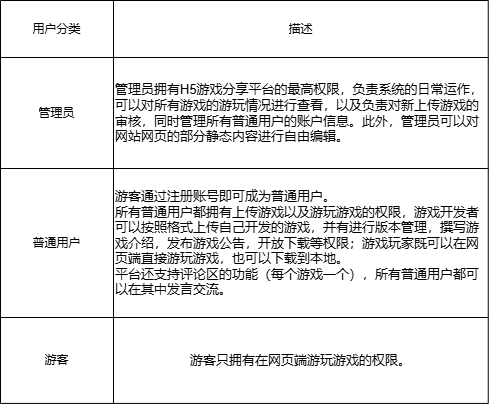
\includegraphics[width=0.8\textwidth]{user_class.png}
  \caption{用户类}
  \label{f1}
\end{figure}


\subsection{产品功能}
产品使用者可分为上述的三种用户,依照各个用户所拥有的权限,H5游戏分享平台的功能如图二所示。

\begin{figure}[htbp]
  \centering
  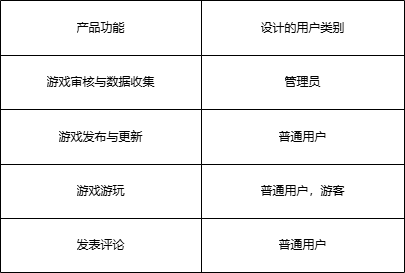
\includegraphics[width=0.8\textwidth]{function.png}
  \caption{产品功能}
  \label{f2}
\end{figure}

\subsection{运行环境}
H5游戏分享平台网站需要通过现代网页浏览器进行访问及操作,较新的浏览器版本可以获得更好的体验。

\subsection{设计和实现上的约束}
系统的设计、编码以及维护将遵照后续提交的《项目总体计划》等文档中的具体要求进行。

在具体设计和实现上,按照以下约束进行:

(1)数据存储

平台采用 drawdb 数据库作为核心数据存储引擎,用于管理用户信息、游戏元数据、评论及交互记录等结构化数据。
数据库设计需满足第三范式(3NF),确保数据一致性和可维护性。

(2)网络服务性能

平台需支持至少100名用户同时在线,并在高峰时段保证核心接口(如游戏加载、用户登录、数据提交)的响应时间不超过1s。

(3)数据安全

完整性保障:
用户上传的游戏文件需要加密,防止在未经授权的情况下被篡改,关键数据的传输可能需要加密。

保密性要求:
用户敏感信息需要加密存储,加密技术必须自动,实时,精确,可靠。可能需要实现安全的第三方登录授权。

可用性限制:
需要通过对使用者的身份验证来防止越权操作,并为合法使用者提供安全便捷的使用。

(4)跨平台兼容性

平台需要兼容主流浏览器的最新版本,并确保HTML5游戏在PC端和移动端的渲染一致性。



\subsection{用户文档}
平台交付时将提供三类用户文档:描述类文档、过程类文档、参考类文档,
旨在帮助用户快速熟悉平台功能,并通过文档高效解决使用中的问题。

(1)描述类文档

描述类文档提供对HTML5游戏分享平台的核心功能、系统架构、界面设计、用户权限及交互特性的全面说明,包括
网站的核心模块(如游戏库、评论区)及其用途,游戏上传/下载、在线试玩、用户评论等功能的具体描述。

(2)过程类文档

过程类文档通过交互式引导和分步教程帮助用户完成关键操作,包括
注册/登录流程等新用户引导,游戏上传/试玩/社交互动等核心功能指引,以及对开发者工具如何使用的提示。

(3)参考类文档

参考类文档按功能模块和常见问题分类,提供精准解决方案,包括了
问题排查指南,网站功能详解,开发者文档,隐私与安全建议。
为用户提供问题的快速解决方案,以便于用户进行操作。


\section{系统功能}
\subsection{用户需求}
% 在这里添加用户需求的内容

\subsection{用例图}
在这里添加用例图的内容

\subsection{功能列表}

\section{类图与 CRC 模型}
\subsection{类图}
% 在这里添加类图的内容

\subsection{CRC 模型}
\subsubsection{User}
% 在这里添加 User 的 CRC 模型


\section{非功能性需求}
\subsection{性能需求}
% 在这里添加性能需求的内容

\subsection{输入要求}
% 在这里添加输入要求的内容


\section{数据流图}

\section{验收准则}
\subsection{功能要求}
% 在这里添加功能要求的内容

\subsection{性能要求}

\subsection{存储要求}
% 在这里添加存储要求的内容

\subsection{维护要求}
% 在这里添加维护要求的内容

\section{UI 原型}

\subsection{登录界面}
% 在这里添加登录界面的内容

\subsection{注册界面}
% 在这里添加注册界面的内容

\subsection{用户主界面}
% 在这里添加用户主界面的内容

\end{document}